% no notes
\documentclass{beamer}
% notes and slides
%\documentclass[notes]{beamer}
% notes only
%\documentclass[notes=only]{beamer}
\usepackage{graphicx} % Allows including images
\usepackage{booktabs} % Allows the use of \toprule, \midrule and \bottomrule in tables
\usepackage{multirow}
\usepackage{multimedia}
\usepackage{circuitikz}
\usepackage{epigraph}
\usepackage{url}
\usepackage[framemethod=tikz]{mdframed}
\usepackage{tikz}
\usetikzlibrary{patterns,shapes.arrows}
\usetikzlibrary{positioning}
\usepackage[framemethod=tikz]{mdframed}
\usepackage{pgfplots}
\pgfplotsset{compat=newest}
\usepgfplotslibrary{groupplots,dateplot}
\usepackage{standalone}
\usepackage{adjustbox}
\usepackage{lmodern}
\usepackage{pgfplots}
\usepackage{amsmath}
\usepackage{amsthm}
\usepackage{multimedia}
\usepackage{standalone}
\usepackage{csquotes}

% python listings
% from https://tex.stackexchange.com/questions/83882/how-to-highlight-python-syntax-in-latex-listings-lstinputlistings-command
% Default fixed font does not support bold face
\DeclareFixedFont{\ttb}{T1}{txtt}{bx}{n}{12} % for bold
\DeclareFixedFont{\ttm}{T1}{txtt}{m}{n}{12}  % for normal

% Custom colors
\usepackage{color}
\definecolor{deepblue}{rgb}{0,0,0.5}
\definecolor{deepred}{rgb}{0.6,0,0}
\definecolor{deepgreen}{rgb}{0,0.5,0}

\usepackage{listings}

% Python style for highlighting
\newcommand\pythonstyle{\lstset{
language=Python,
basicstyle=\ttm,
morekeywords={self},              % Add keywords here
keywordstyle=\ttb\color{deepblue},
emph={MyClass,__init__},          % Custom highlighting
emphstyle=\ttb\color{deepred},    % Custom highlighting style
stringstyle=\color{deepgreen},
frame=tb,                         % Any extra options here
showstringspaces=false
}}


% Python environment
\lstnewenvironment{python}[1][]
{
\pythonstyle
\lstset{#1}
}
{}

% Python for external files
\newcommand\pythonexternal[2][]{{
\pythonstyle
\lstinputlisting[#1]{#2}}}

% Python for inline
\newcommand\pythoninline[1]{{\pythonstyle\lstinline!#1!}}

\definecolor{cyan}{RGB}{42,161,152}
\definecolor{violet}{RGB}{108,113,196}
\definecolor{red}{RGB}{220,50,47}

\PassOptionsToPackage{american}{babel} % change this to your language(s), main language last
% Spanish languages need extra options in order to work with this template
% \PassOptionsToPackage{spanish,es-lcroman}{babel}
\usepackage{babel}

\PassOptionsToPackage{%
  backend=biber,bibencoding=utf8, %instead of bibtex
  %backend=bibtex8,bibencoding=ascii,%
  language=auto,%
  style=numeric-comp,%
  %style=authoryear-comp, % Author 1999, 2010
  %bibstyle=authoryear,dashed=false, % dashed: substitute rep. author with ---
  style=alphabetic,
  sorting=nyt, % name, year, title
  maxbibnames=10, % default: 3, et al.
  %backref=true,%
  %natbib=true % natbib compatibility mode (\citep and \citet still work)
}{biblatex}
\usepackage{biblatex}

\addbibresource{bib.bib}

\usetheme{metropolis}           % Use metropolis theme
\setbeamertemplate{caption}[default]
\title{Introduction to Convolutional Neural Networks}
\date{\today}
\institute{High Performance Computing and Analytics Lab, University of Bonn}
\author{Moritz Wolter}

\titlegraphic{
\includegraphics[width=2.00cm]{UNI_Bonn_Logo_Standard_RZ.pdf}}
\begin{document}
    \maketitle

    \begin{frame}
    \frametitle{Overview} 
    \tableofcontents
    \end{frame}

    \begin{frame}{Motivation \cite{goodfellow2016deep}}
        \begin{itemize}
            \item sparse interactions
            \item parameter sharing
            \item equivariant representations (i.e. with respect to translation)
            \item efficiency
            \item Train deeper networks.
        \end{itemize}
        \note{
            Sparse interactions: From dense to block circulant matrix. \\
            Parameter sharing: Use the same parameters for more than one job. \\
            Equvariance: Translations of an input should not change the outcome.
        }
    \end{frame}

    \begin{frame}{The invention of convolutional neural networks}
        Proposed in Yann le Cun's \cite{lecun1989handwritten}.
        
        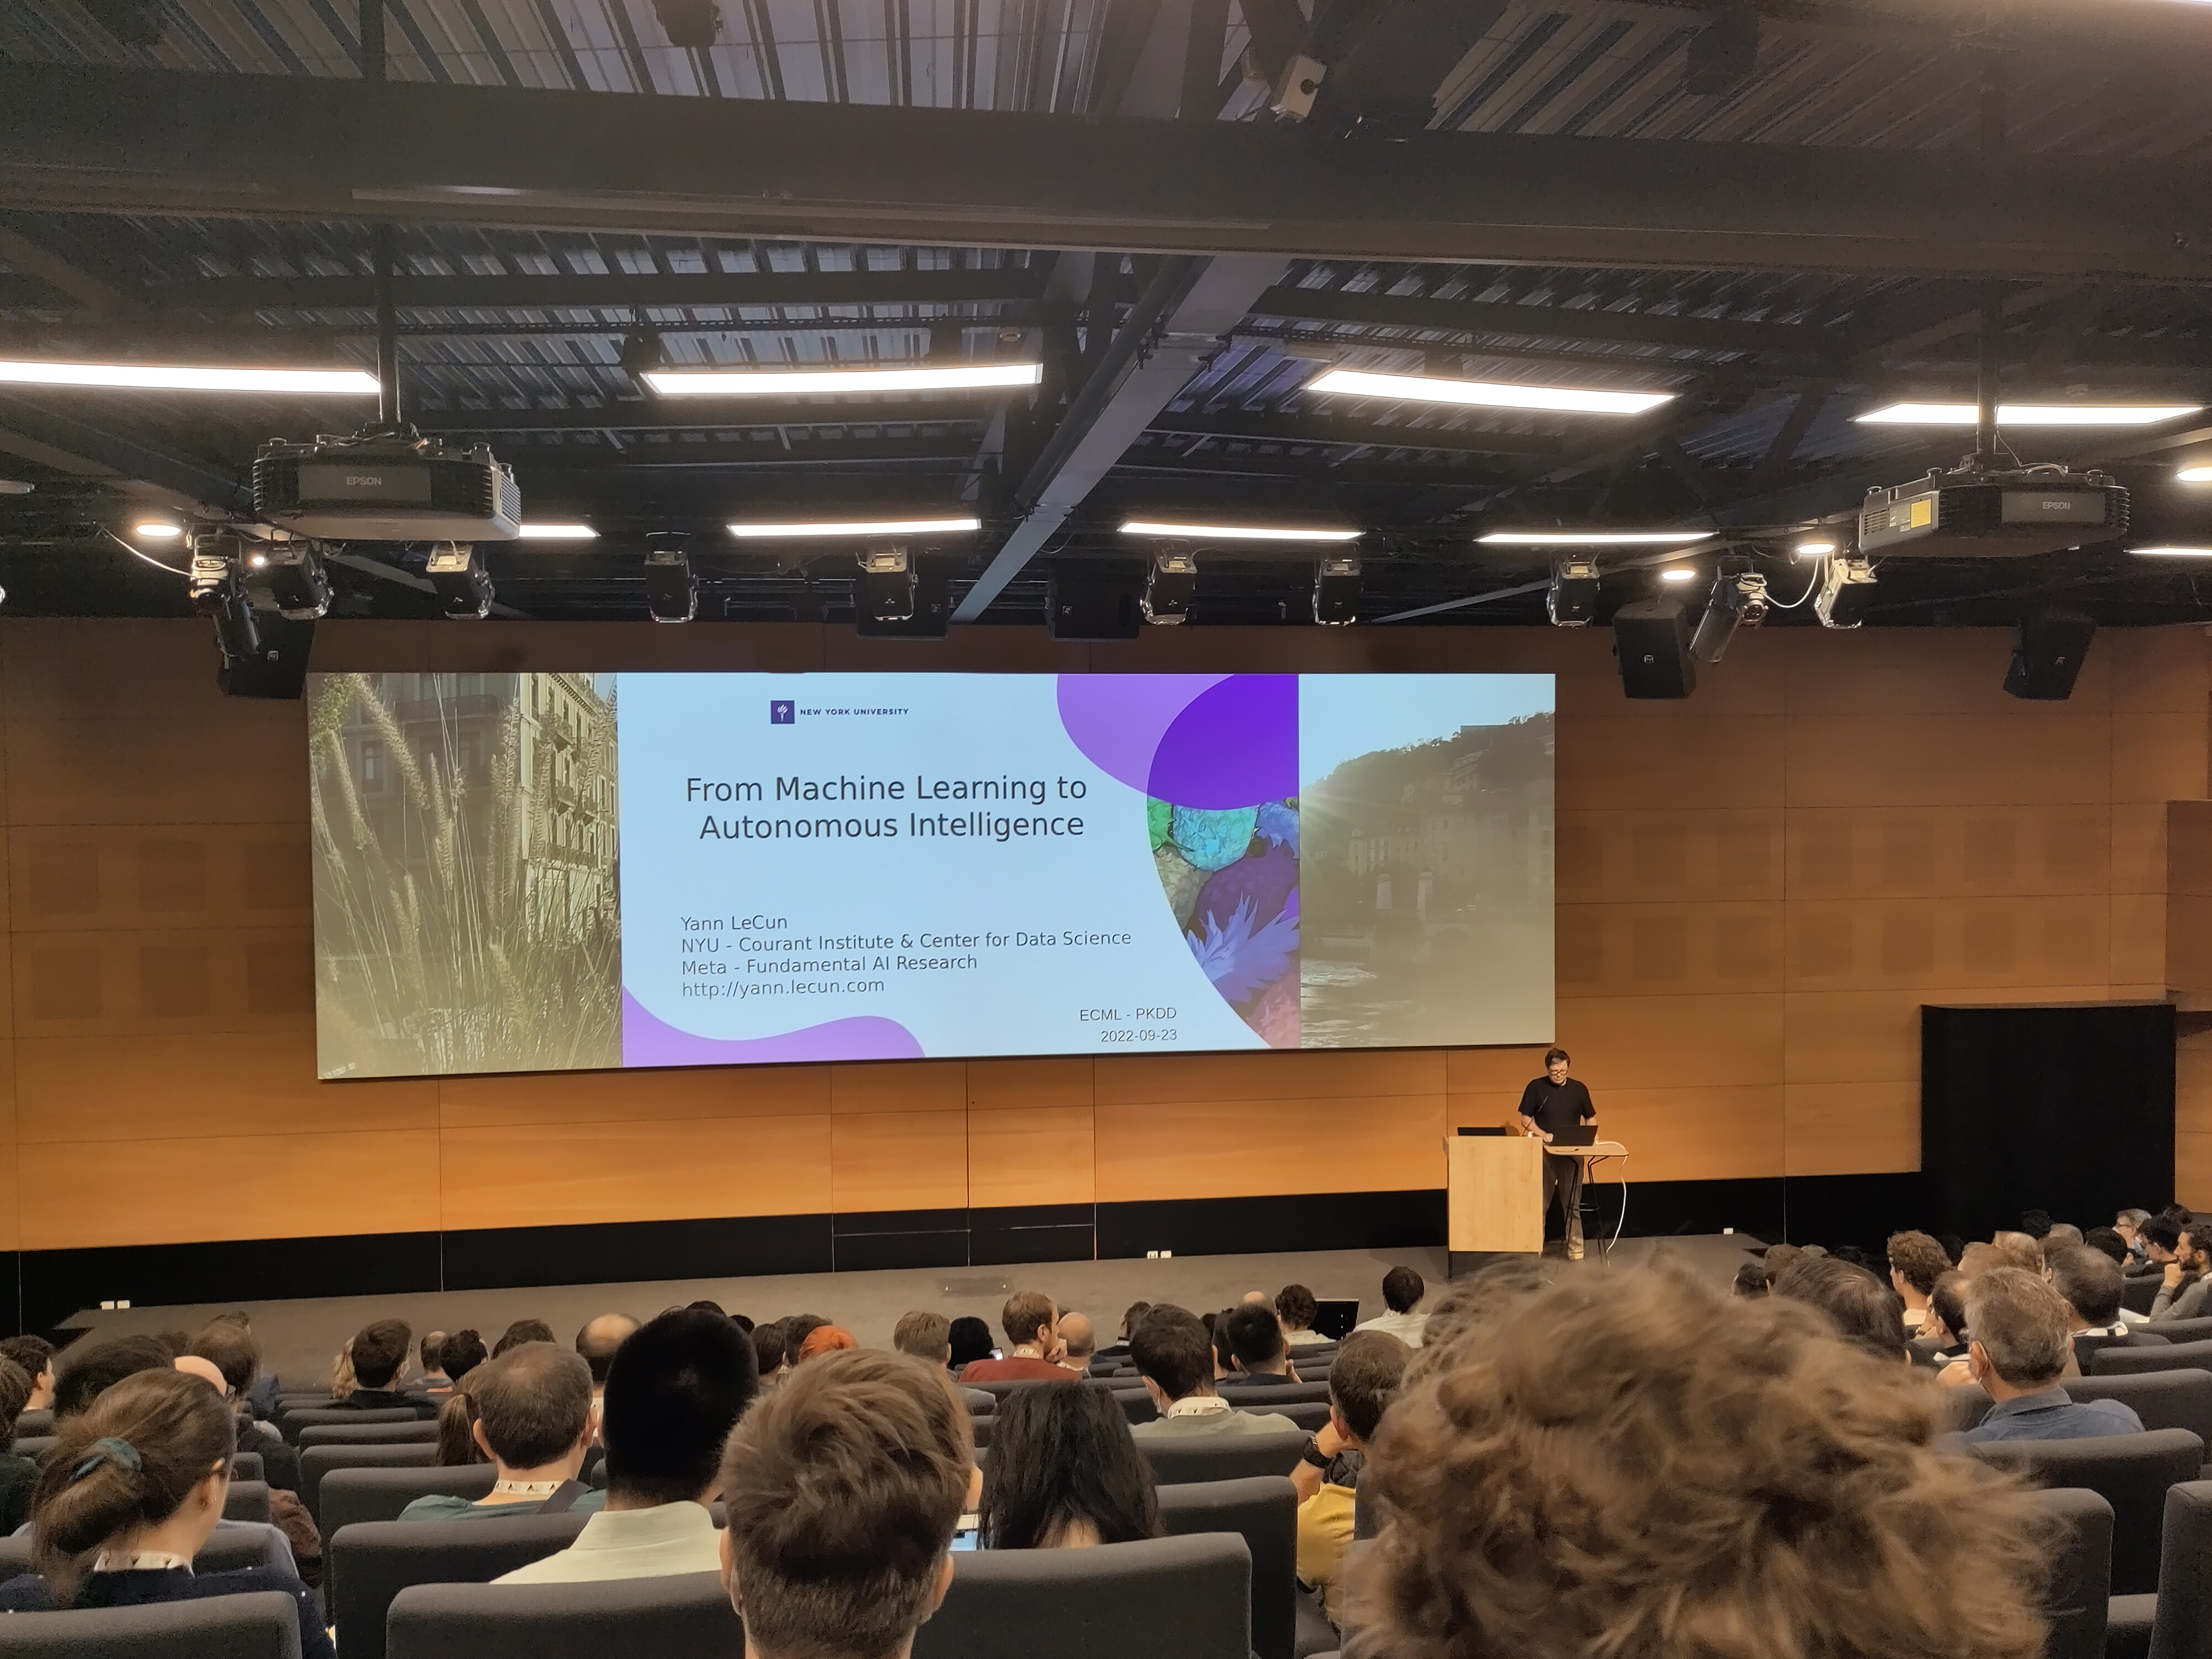
\includegraphics[width=.8\linewidth]{figures/IMG_20220923_090433.jpg}
    \end{frame}


    \section{The convolution operation in machine learning}

    \begin{frame}{Defining convolution}
        For two one-dimensional signals $x \in \mathbb{R}^T$
        and $k \in \mathbb{R}^T$, convolution is defined as
        \begin{align}
            s(t) = (x * k)(t) = \sum_{a=0}^{T} x(a)k(t - a),
        \end{align}
        for numbers $t,a$. Possible $t$ will depend on signal length and padding. \\
        In 2D, we require a kernel matrix $K \in \mathbb{R}^{O,P}$ and a image matrix
        $I \in \mathbb{K}^{N,M}$
        \begin{align}
            S(i,j) = (K * I)(i,j) = \sum_m^M \sum_n^N I(i-m, j-n)K(n,m)
        \end{align}
        Again not just any $i,j$ will do. We will see what this means in a minute.
    \end{frame}


    \begin{frame}{Defining cross-correlation}
        
        \begin{align}
            S(i,j) = (K*I) = \sum_m^M \sum_n^N I(i+m, j+n)K(m,n)
        \end{align}
        Cross-correlation is convolution without flipping the kernel \cite{goodfellow2016deep}.
        Many machine-learning libraries implement cross-correlation and
        call it convolution. In this course we will follow their example.
    \note{
        A convolution example on the board: 
        \begin{align}
            \mathbf{I} = \begin{pmatrix}
                1 & 3 & -1 \\
                2 & 1 &  0 \\
                0 & 2 & -1 \\
            \end{pmatrix},
            \mathbf{K} = \begin{pmatrix}
                1 & 0 \\
                2 & -1 \\
            \end{pmatrix}
        \end{align}
        Computing $\mathbf{I}*\mathbf{K}$:
        \begin{align}
            \mathbf{I}*\mathbf{K} &= \begin{pmatrix}
                1\cdot 1 + 3\cdot 0 + 2\cdot 2 + 1\cdot (-1) & 3\cdot 1 + (-1)\cdot 0 + 1\cdot 2 + 0\cdot (-1) \\
                2\cdot 1 + 1\cdot 0 + 0\cdot 2 + 2\cdot (-1) & 1\cdot 1 + 0\cdot 0 + 2\cdot 2 + (-1)\cdot (-1)  
            \end{pmatrix} \\
            &= \begin{pmatrix}
                4 & 5 \\
                0 & 6
            \end{pmatrix}
        \end{align}
    }
    \end{frame}

    \begin{frame}{Illustrating the convolution operation}
        \begin{figure}
            \centering
            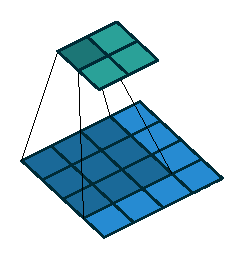
\includegraphics[scale=0.7]{./figures/no_padding_no_strides_00.pdf}
            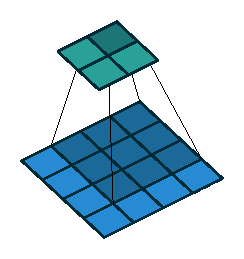
\includegraphics[scale=0.7]{./figures/no_padding_no_strides_01.pdf} \\
            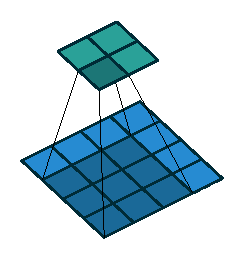
\includegraphics[scale=0.7]{./figures/no_padding_no_strides_02.pdf}
            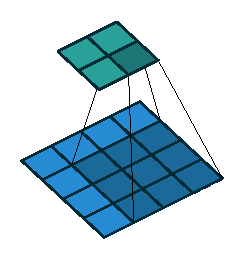
\includegraphics[scale=0.7]{./figures/no_padding_no_strides_03.pdf}
            \caption{Illustration of the convolution operation without padding and unit strides \cite{dumoulin2016guide}.}
        \end{figure}
    \end{frame}

    \begin{frame}{Strided convolution}
        \begin{figure}
            \centering
            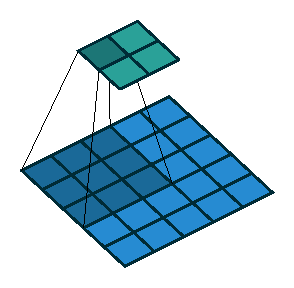
\includegraphics[width=0.25\linewidth]{./figures/no_padding_strides_00.pdf}
            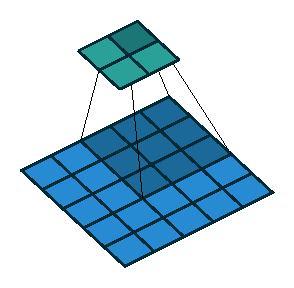
\includegraphics[width=0.25\linewidth]{./figures/no_padding_strides_01.pdf} \\
            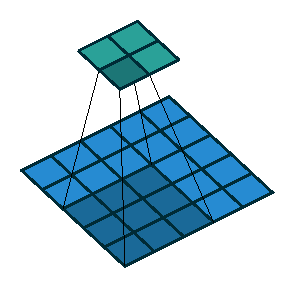
\includegraphics[width=0.25\linewidth]{./figures/no_padding_strides_02.pdf}
            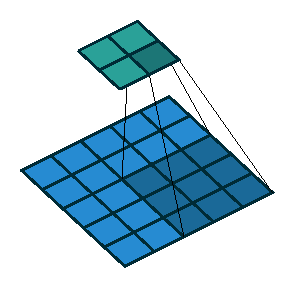
\includegraphics[width=0.25\linewidth]{./figures/no_padding_strides_03.pdf}
            \caption{Visualization of stride two convolutions without padding \cite{dumoulin2016guide}.}
        \end{figure}
    \end{frame}

    \begin{frame}{Padded convolution}
        \begin{figure}
            \centering
            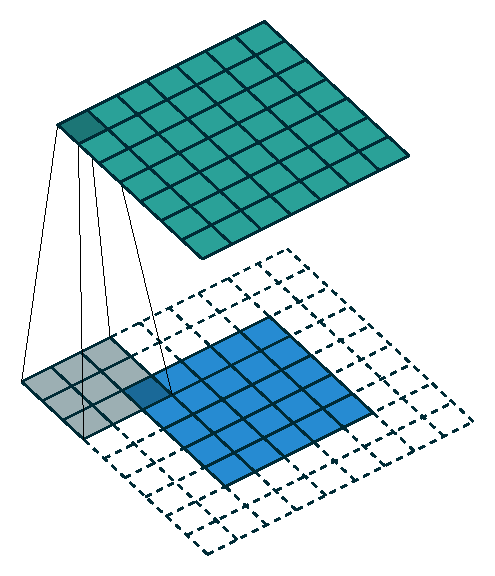
\includegraphics[width=0.25\linewidth]{./figures/full_padding_no_strides_00.pdf}
            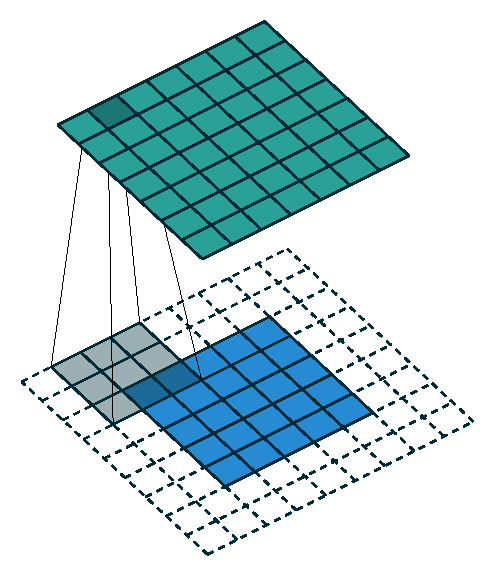
\includegraphics[width=0.25\linewidth]{./figures/full_padding_no_strides_01.pdf} \\
            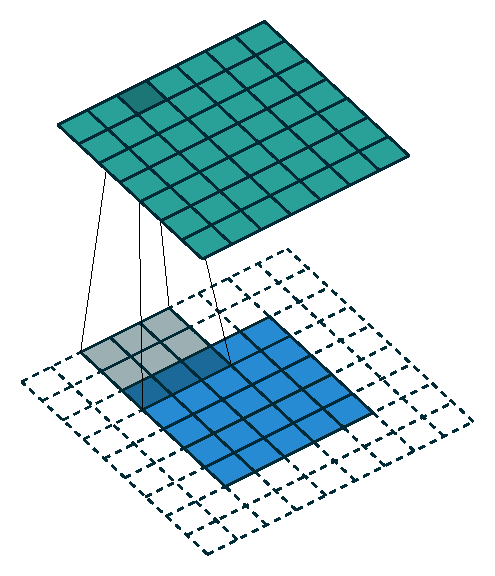
\includegraphics[width=0.25\linewidth]{./figures/full_padding_no_strides_02.pdf}
            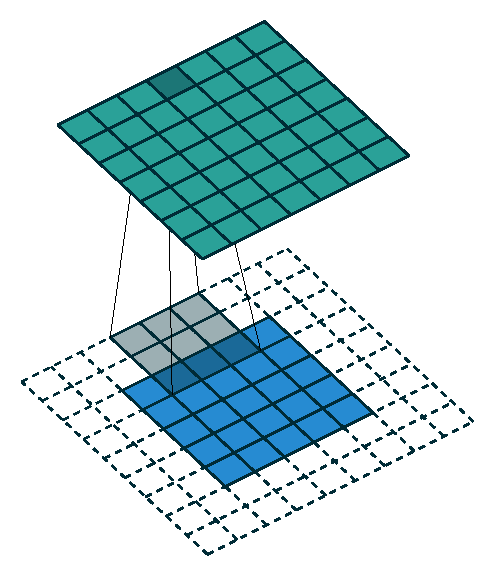
\includegraphics[width=0.25\linewidth]{./figures/full_padding_no_strides_03.pdf}
            \caption{Visualization of fully padded convolutions with unit strides \cite{dumoulin2016guide}.}
        \end{figure}
    \end{frame}

    \begin{frame}{Summary}
        \begin{itemize}
            \item The convolution operation slides convolution kernels over an image.
            \item Padding avoids losing pixels on the side.
            \item Strided convolutions downsample the input.
            \item Moving in steps of two pixels, for example, cuts the resolution in half.
        \end{itemize}
    \end{frame}

    \section{Understanding convolution}

    \begin{frame}{Getting computers to find Waldo}
        \begin{figure}
            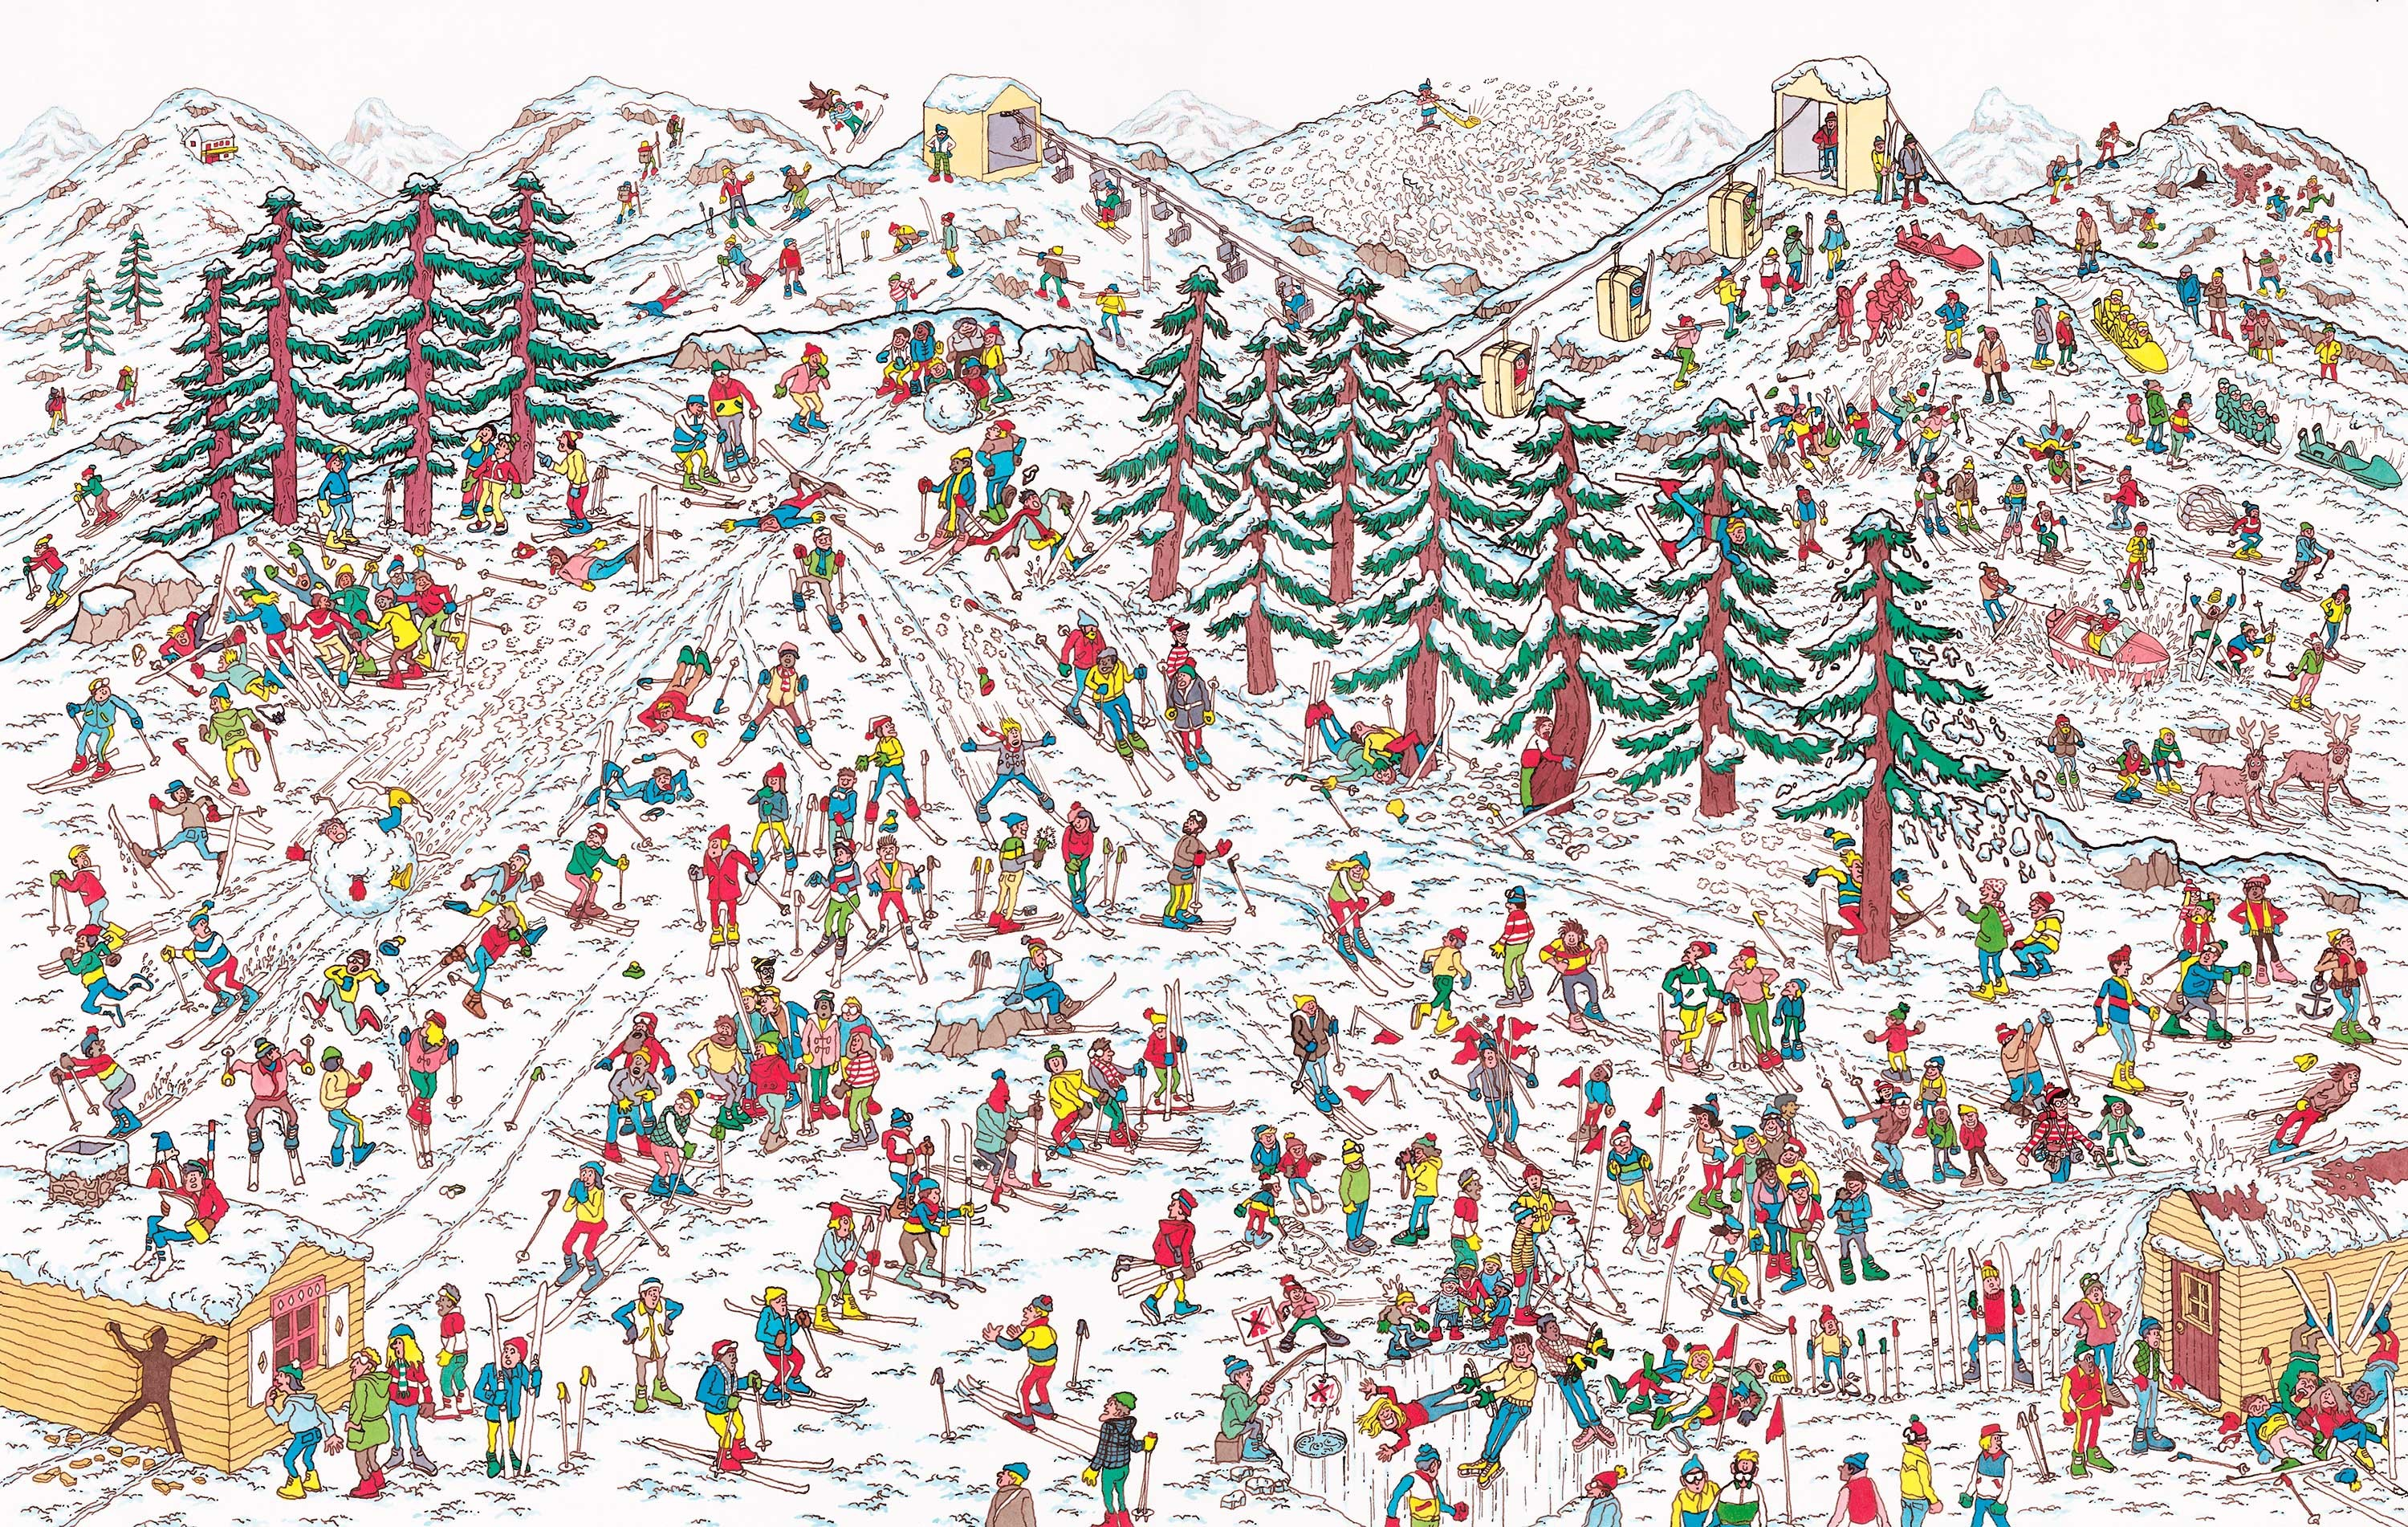
\includegraphics[scale=0.1]{./python/waldo_snow.jpg}
            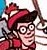
\includegraphics{./python/waldo_small.jpg}
        \end{figure}
    \end{frame}

    \begin{frame}{Finding Waldo via cross-correlation.}
        \begin{figure}
        \centering
        \includestandalone[scale=1]{./figures/corr_plot}
        %\caption{}
        \end{figure}
    \end{frame}

    \begin{frame}{Summary}
        \begin{itemize}
            \item Cross-correlation is called convolution in the machine learning literature.
            \item Patterns can be located in signals via cross-correlation.
        \end{itemize}
    \end{frame}

    \section{Convolutional neural networks}
    \begin{frame}{Motivating convolutional neural networks (CNN)}
        \begin{itemize}
            \item Fixed filters work if we are looking for a very specific waldo.
            \item In other cases, we need a better solution.
            \item Convolutional neural networks rely on filter optimization via back-propagation.
            \item Filter optimization turns CNNs into very versatile tools!
        \end{itemize}
    \end{frame}

    \begin{frame}{Multichannel convolution}
        \begin{figure}
            \includestandalone[width=.8\linewidth]{./figures/cnn_channels}
            \caption{The plot shows a convolution
            computation using a $3x2x3x3$ kernel on a $2x5x5$ input.
            The kernel pairs convolve with the input, producing $3x3$ results.
            $+$ adds the two channels for each of the three tensors.
            Finally, everything is stacked. Inspired by \cite[page 9]{dumoulin2016guide}. }
        \end{figure}
        \note{
            On the board:
            Explain the effect of the input and output shapes. \\
            I.e.: \\
                Kernel $(O,I,H,W)$:  Out-Channels, In-Channels, Height, Width \\
                Image  $(N,C,H,W)$: Batch-Size, Channels, Height, Width \\
                Results in: \\
                Result $(N,O, H_n, W_n)$ 
        }
    \end{frame}

    \begin{frame}{Computing the output shape of a CNN layer}
        One can determine the output shape for each dimension individually.
        Without zero padding and a stride size of one,
        \begin{align}
            o = (i-k) + 1
        \end{align}
        can be used to compute the output size. $i$ denotes the input size,
        and $k$ is the kernel size. \cite{dumoulin2016guide} covers all cases which appear in practice.
    \end{frame}

    \begin{frame}{Image to column and the forward pass}
        We already know how to train dense network layers using matrix multiplication.
        Training a CNN the same way requires restructuring the image to express convolution as matrix multiplication,
        \begin{align}
            \overline{\mathbf{h}} &= \mathbf{K}_f \mathbf{v}_I  + \mathbf{b}, \\ 
            \mathbf{h}_f &= f(\overline{\mathbf{h}}).
        \end{align}
        $\mathbf{v}_I \in \mathbb{R}$ denotes the restructured image input. $\mathbf{K}_f \in \mathbb{R}^{k_o, k_i \cdot k_h \cdot k_w}$ the flattened restructured kernel.
        $o,i,h,w$ denote the output, input, height, and width dimensions, respectively.
        \note{
            im2col demonstrate on the board:
            Idea: collect the image convolution patches in the columns of a matrix. Use python indexing to set it up.
            For a $3 \times 3$ matrix and a $2 \times 2$ kernel without padding this would lead to the index matrices: 
            \begin{align}
                \begin{pmatrix}
                    0 & 1 & 2 \\
                    3 & 4 & 5 \\
                    6 & 7 & 8 \\
                \end{pmatrix}
                \rightarrow
                \begin{pmatrix}
                0 & 1 & 3 & 4 \\
                1 & 2 & 4 & 5 \\
                3 & 4 & 6 & 7 \\
                4 & 5 & 7 & 8
                \end{pmatrix}
            \end{align}
        }
    \end{frame}

    \begin{frame}{The backward pass}
        We apply the rules for dense layers to the restructured convolutional layer data,
        \begin{align} 
            \delta \mathbf{K}_f &= [f'(\overline{\mathbf{h}}) \odot \triangle]_f \mathbf{v}^T_I,  &  
            \delta \mathbf{b} &= f'(\overline{\mathbf{h}}) \odot \triangle,   \\  
            \delta \mathbf{x} &= \big(\mathbf{K}_f^T [f'(\overline{\mathbf{h}}) \odot \triangle]_f \big)_{I^{-1}}.
        \end{align}
        With $I$ and $I^{-1}$ denoting the \texttt{im2col} and \texttt{col2im} operations.
        All major deep learning frameworks have both operations built in.
    \end{frame}

    \begin{frame}{The classifier at the end}
        \begin{figure}
        \includestandalone[width=\linewidth]{./figures/cnn}
        \caption{The LeNet-architecture\cite{lecun1989handwritten} as illustrated by \cite{StutzCNN}.}
        \end{figure}
    \end{frame}

    \begin{frame}{The shifting input problem}
        \begin{itemize}
            \item With the tools we have seen, shifting an input also shifts the CNN output before the dense classifier.
            \item Shifting the input would shift the input in front of the final dense-classifier neurons.
            \item We want invariance to translation.
        \end{itemize}
    \end{frame}


    \begin{frame}{Pooling}
        Max pooling layers choose maximum values in predefined regions.
        Two by two max pooling, for example, picks the maximum in neighboring areas of four pixels.
        If an input is shifted by two pixels, the result will remain the same!
        Pooling layers are used repeatedly for a cumulative effect.
        \note{
            $\rightarrow $ Draw the effect of max pooling on the board.
        }
    \end{frame}

    \begin{frame}{MNIST}
        \begin{figure}
            \includestandalone[height=1cm, width=6cm]{./figures/mnist_sequence}
            \caption{Sample digits from the MNIST-database.}
        \end{figure}
        \begin{figure}
            \includestandalone[scale=.6]{./figures/cnn_mnist}
            \caption{Mean convergence of two-layer CNN with a dense classifier.}
        \end{figure}
    \end{frame}

    \begin{frame}{Deep convolutional neural networks}
        \begin{figure}
            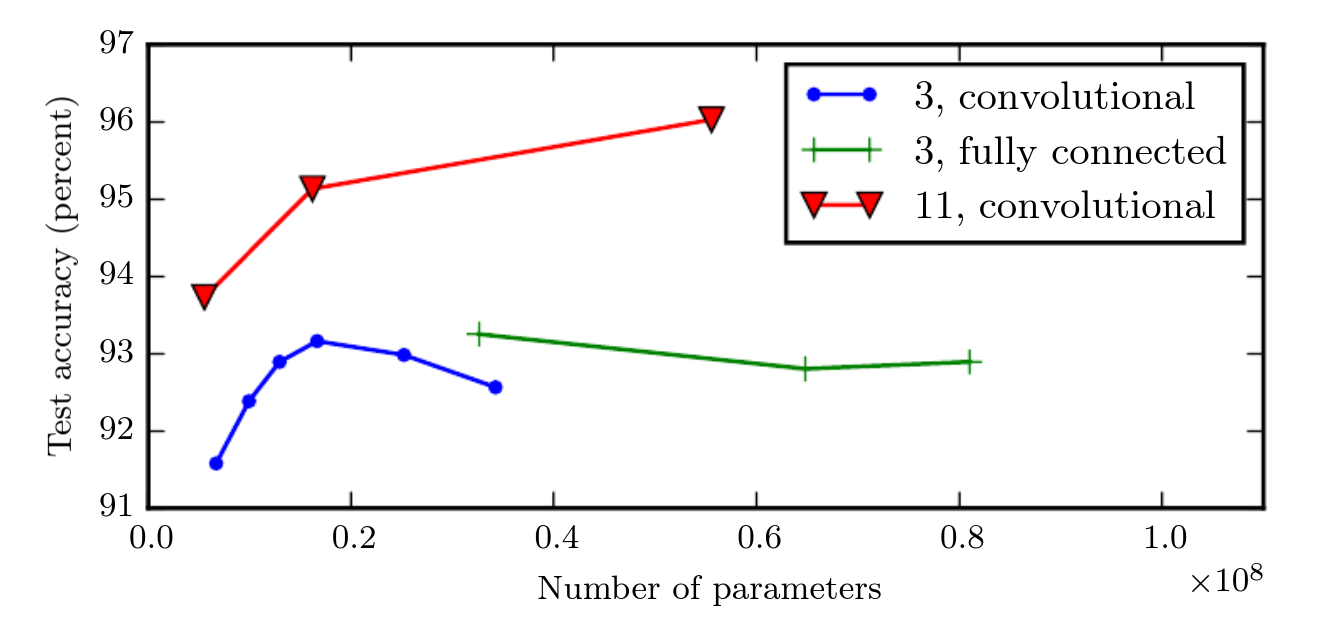
\includegraphics[width=0.8\linewidth]{figures/deep_cnn.png}
            \caption{Comparing deep networks with and without convolutional structures on the Google-Street view dataset
                \cite[page 199]{goodfellow2016deep}.}
        \end{figure}
        \note{ \cite{goodfellow2016deep} tells us: \\ 
        Effect of number of parameters. Deeper models tend to perform better.
        This is not merely because the model is larger. This experiment from Goodfellow et al.
        (2014d) shows that increasing the number of parameters in layers of convolutional networks
        without increasing their depth is not nearly as effective at increasing test set performance,
        as illustrated in this figure.}
    \end{frame}


    \begin{frame}[allowframebreaks]{Literature}
        \printbibliography
    \end{frame}
    
\end{document}
